\documentclass[14pt,pdf,hyperref={unicode}]{beamer}

% \documentclass[aspectratio=43]{beamer}
% \documentclass[aspectratio=1610]{beamer}
% \documentclass[aspectratio=169]{beamer}

\usepackage{lmodern}

% подключаем кириллицу 
\usepackage[T2A]{fontenc}
\usepackage[utf8]{inputenc}
\usepackage{listings}
\usepackage{graphicx}
\usepackage{hyperref}

% отключить клавиши навигации
\setbeamertemplate{navigation symbols}{}

% тема оформления
\usetheme{CambridgeUS}

% цветовая схема
\usecolortheme{seahorse}

\definecolor{light-gray}{gray}{0.90}

\lstset{basicstyle=\ttfamily,breaklines=true}

\title{Семинар №10}   
\subtitle{ФАКИ \the\year}
\author{Бирюков В. А.} 
\date{\today} 
% \logo{
\includegraphics[height=5mm]{images/logo.png}\vspace{-7pt}}

\begin{document}

\lstset{language=C}

% титульный слайд
\begin{frame}
\titlepage
\end{frame} 

\defverbatim[colored]\makeset{
\begin{lstlisting}[language=C++,basicstyle=\ttfamily,keywordstyle=\color{blue}]
void make_set(int X) {
  parent[X] = X;
}
\end{lstlisting}
}

\lstset{
  language=C,                % choose the language of the code
  keywordstyle=\color{blue},
  numbers=none,                   % where to put the line-numbers
  stepnumber=1,                   % the step between two line-numbers.        
  numbersep=5pt,                  % how far the line-numbers are from the code
  backgroundcolor=\color{light-gray},  % choose the background color. You must add \usepackage{color}
  showspaces=false,               % show spaces adding particular underscores
  showstringspaces=false,         % underline spaces within strings
  showtabs=false,                 % show tabs within strings adding particular underscores
  tabsize=2,                      % sets default tabsize to 2 spaces
  captionpos=b,                   % sets the caption-position to bottom
  breaklines=true,                % sets automatic line breaking
  breakatwhitespace=true,         % sets if automatic breaks should only happen at whitespace
}






\section{Алгоритмы}
\begin{frame}
\begin{center}
\begin{beamercolorbox}[sep=8pt,center]{part
title}
\usebeamerfont{part title}\insertsection
\end{beamercolorbox}
\end{center}
\end{frame}




\begin{frame}[fragile]
\frametitle{Алгоритм} 
\begin{itemize}
\item Алгоритм -- это формально описанная вычислительная процедура, получающая исходные данные, и выдающая результат
вычислений на выход \\
(Кормен и др. "Алгоритмы: построение и анализ")
\end{itemize}
\end{frame}



\begin{frame}[fragile]
\frametitle{Задача сортировки} 
\begin{itemize}
\item Задана последовательность чисел \\
\item Нужно найти такую перестановку исходной последовательности, чтобы элементы были расположены по возрастанию  \\
\item 5 2 4 6 1 3 2 9  $\rightarrow$ 1 2 2 3 4 5 6 9
\end{itemize}
\end{frame}


\begin{frame}[fragile]
\frametitle{Простейшие сортировки} 
\begin{itemize}
\item Сортировка вставками \\
\item Сортировка выбором \\
\item Сортировка пузырьком \\
\end{itemize}
\end{frame}


\section{Анализ алгоритмов}
\begin{frame}
\begin{center}
\begin{beamercolorbox}[sep=8pt,center]{part
title}
\usebeamerfont{part title}\insertsection
\end{beamercolorbox}
\end{center}
\end{frame}

\begin{frame}[fragile]
\frametitle{Анализ алгоритмов} 
\begin{itemize}
\item Обычно изучают зависимость времени работы от размера входа \\
\item Размер входа -- зависит от конкретной задачи \\
\item Для сортировки, размер входа -- это количество элементов, которые нужно отсортировать \\
\item Время работы -- число элементарных шагов, которые выполняет алгоритм
\end{itemize}
\end{frame}

\begin{frame}[fragile]
\frametitle{Пример анализа} 
\framesubtitle{Сортировка пузырьком}
\begin{lstlisting}[language=C++,basicstyle=\ttfamily,keywordstyle=\color{blue}]
for (int j = 0; j < length-1; j++)
    for (int i = 0; i < length-1; i++)
         if (a[i] > a[i+1])
             swap(a[i], a[i+1]);
\end{lstlisting}
\begin{itemize}
\item Число операций, требуемых на один проход: $a * n$\\
\item Число проходов: $n$\\
\item Значит, время работы $\sim n^2$\\
\end{itemize}

\end{frame}


\section{Принцип "разделяй и влавствуй"}
\begin{frame}
\begin{center}
\begin{beamercolorbox}[sep=8pt,center]{part
title}
\usebeamerfont{part title}\insertsection
\end{beamercolorbox}
\end{center}
\end{frame}

\begin{frame}[fragile]
\frametitle{Принцип "разделяй и влавствуй"} 
\begin{itemize}
\item Задача разбивается на несколько подзадач меньшего размера \\
\item Эти задачи решаются (обычно с помощью рекурсивного вызова) \\
\item Решения этих задач комбинируются и получается решение исходной задачи \\
\end{itemize}
\end{frame}

\begin{frame}[fragile]
\frametitle{Принцип "разделяй и влавствуй" для сортировки} 
\frametitle{Сортировка слиянием} 
\begin{itemize}
\item Разбиваем массив на 2 половины \\
\item Сортируем каждую половину \\
\item Соединяем 2 упорядоченных массива в один \\
\end{itemize}
\end{frame}

\begin{frame}[fragile]
\frametitle{Сортировка слиянием} 
\begin{center}
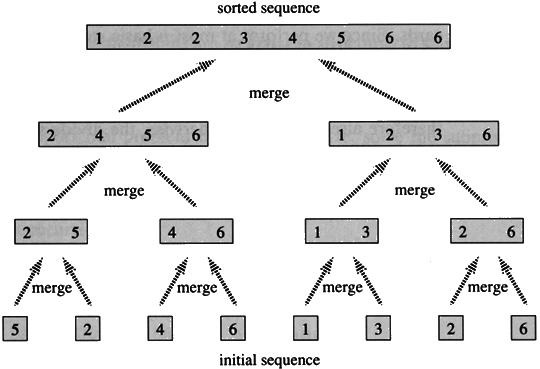
\includegraphics[width=0.9\linewidth]{images/mergeSort.png}
\end{center}
\end{frame}


\begin{frame}[fragile]
\frametitle{Сортировка слиянием} 
\begin{center}
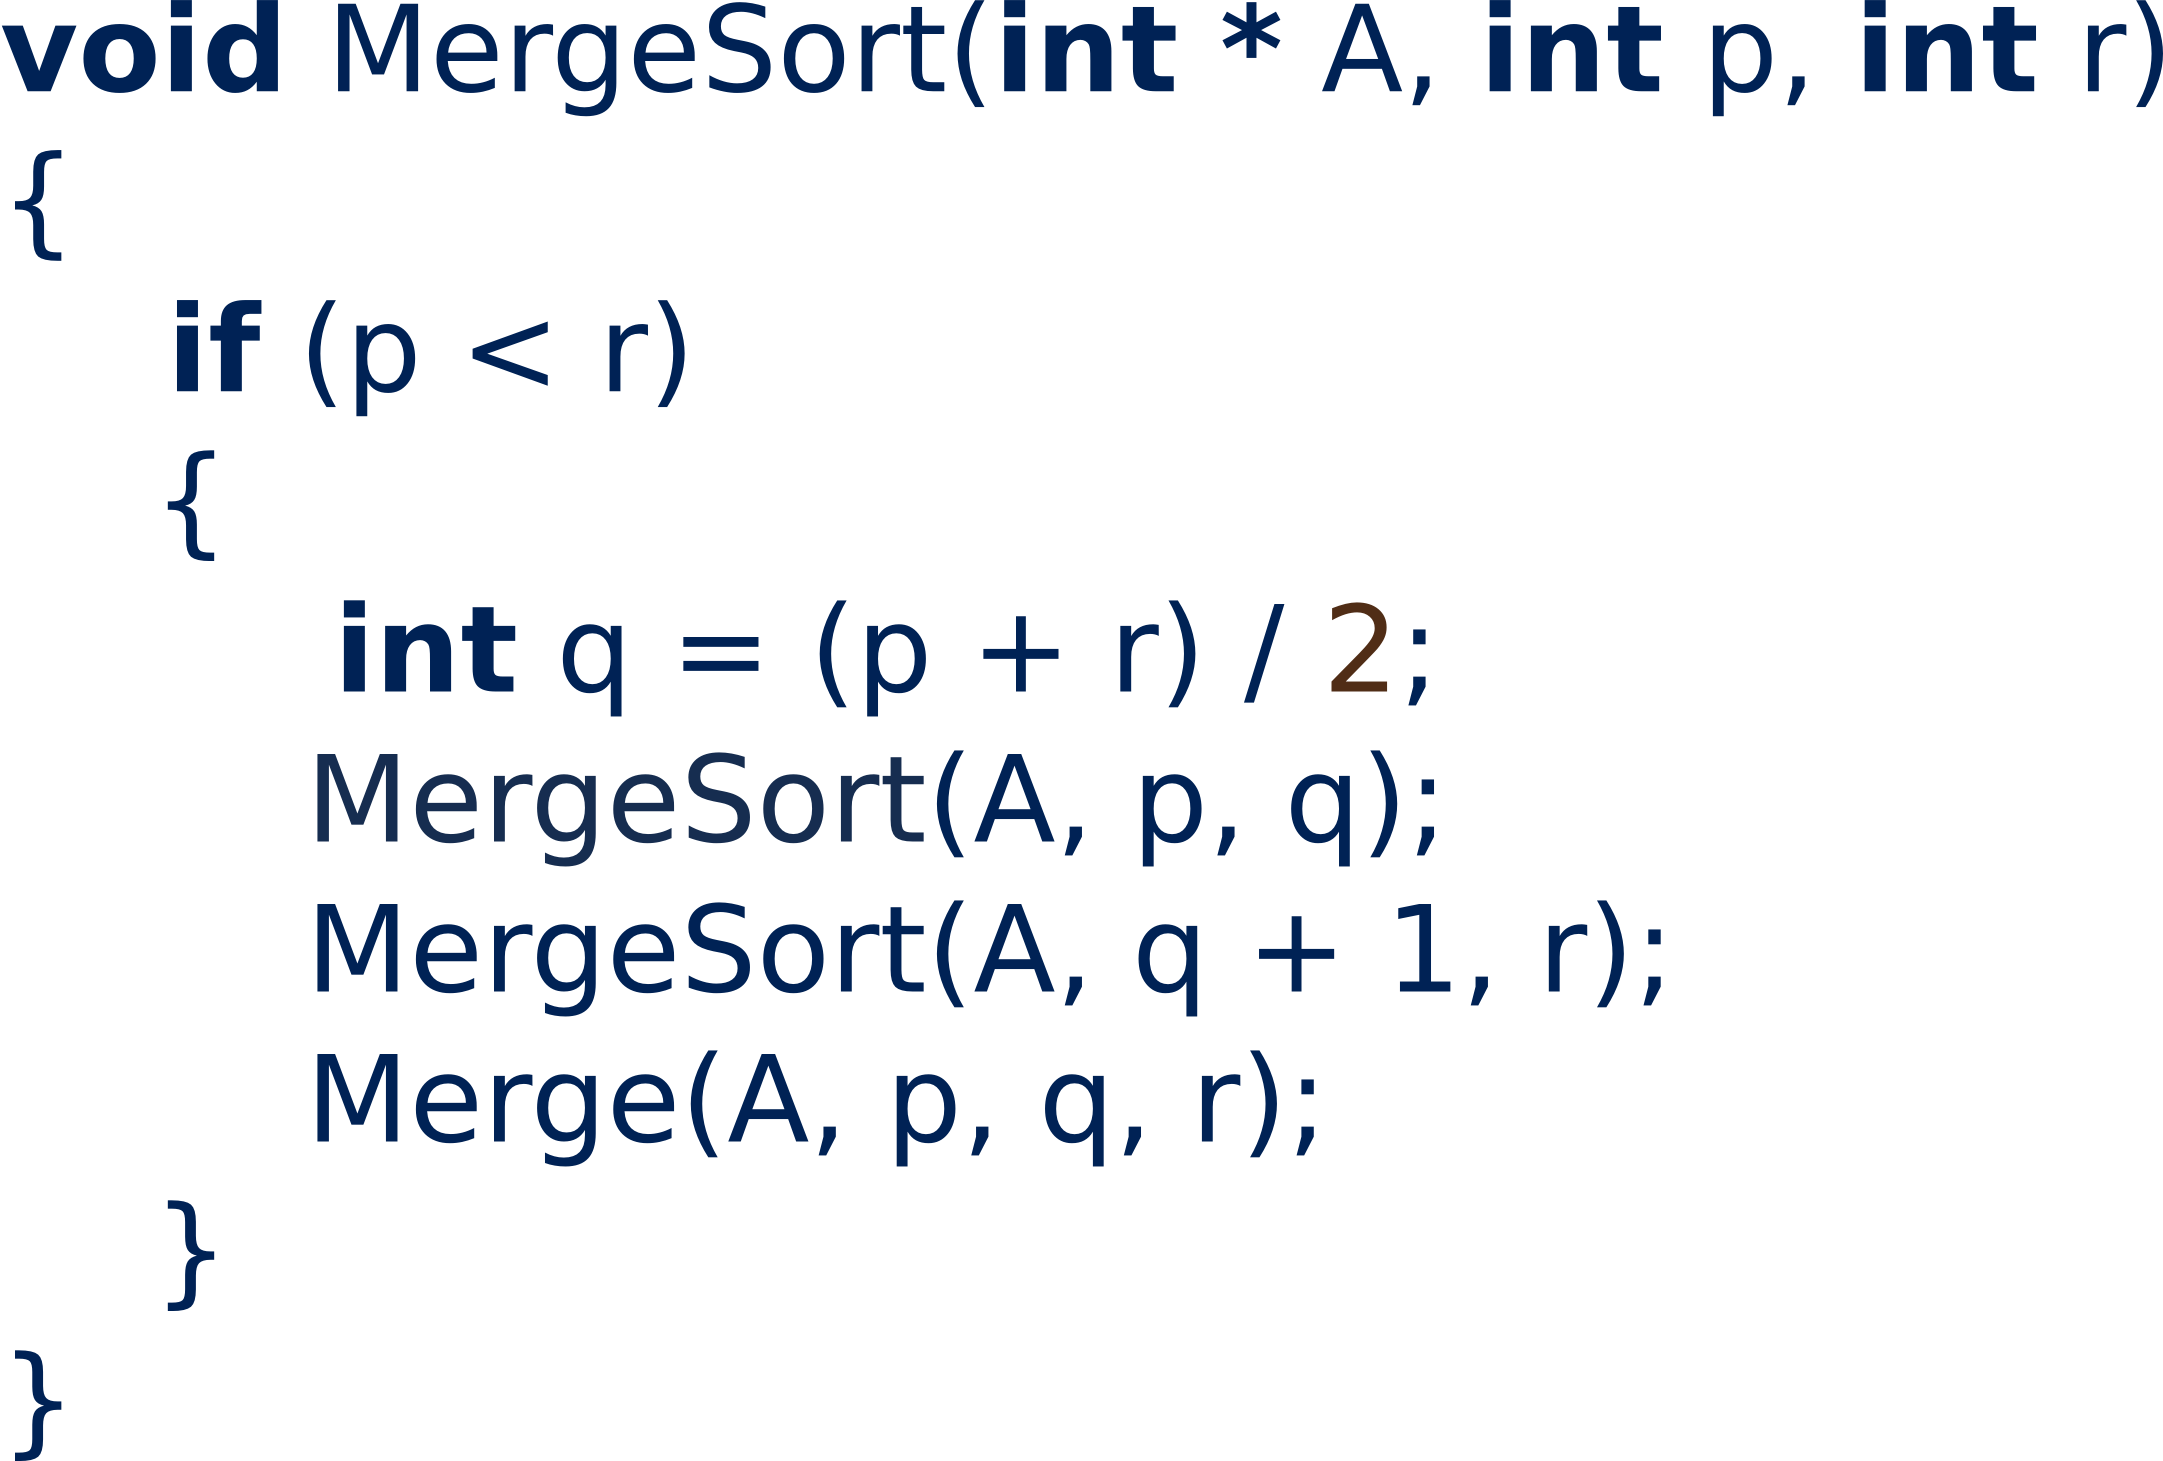
\includegraphics[width=0.9\linewidth]{images/mergeSort_pseudo.png}
\end{center}
\end{frame}



\section{Быстрая сортировка}
\begin{frame}
\begin{center}
\begin{beamercolorbox}[sep=8pt,center]{part
title}
\usebeamerfont{part title}\insertsection
\end{beamercolorbox}
\end{center}
\end{frame}


\begin{frame}[fragile]
\frametitle{Принцип "разделяй и влавствуй" для сортировки} 
\frametitle{Быстрая cортировка (quicksort)} 
\begin{itemize}
\item Выбираем в массиве некоторый элемент, который будем называть опорным \\
\item Переставляем элементы массива таким образом, чтобы все элементы со значением меньшим или равным опорному элементу, оказались слева от него, а все элементы, превышающие по значению опорный — справа от него \\
\item Рекурсивно сортируем подмассивы, лежащие слева и справа от опорного элемента\\
\end{itemize}
\end{frame}

\begin{frame}[fragile]
\frametitle{Быстрая cортировка (quicksort)} 
\begin{center}
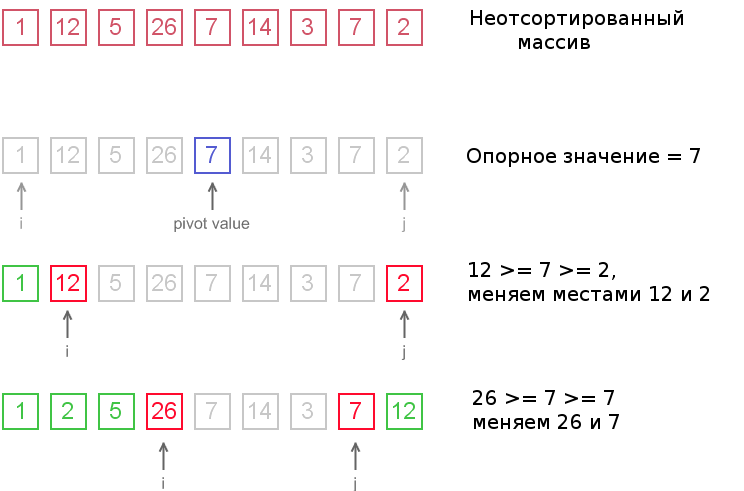
\includegraphics[width=0.9\linewidth]{images/qs1.png}
\end{center}
\end{frame}

\begin{frame}[fragile]
\frametitle{Быстрая cортировка (quicksort)} 
\begin{center}
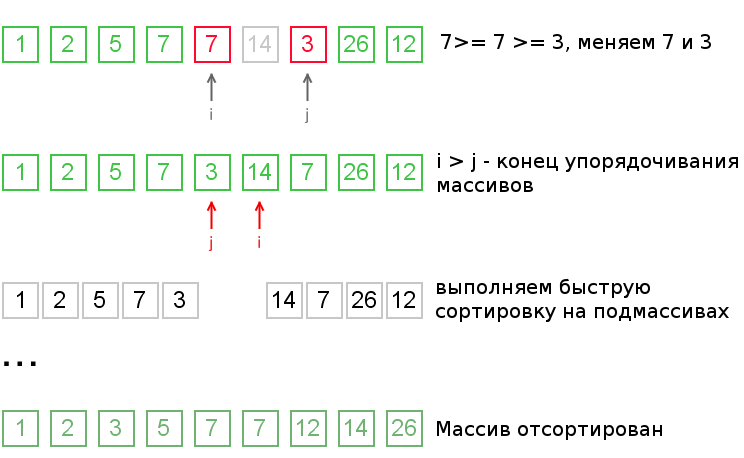
\includegraphics[width=0.9\linewidth]{images/qs2.png}
\end{center}
\end{frame}


\section{Время работы сортировок}
\begin{frame}
\begin{center}
\begin{beamercolorbox}[sep=8pt,center]{part
title}
\usebeamerfont{part title}\insertsection
\end{beamercolorbox}
\end{center}
\end{frame}

\begin{frame}[fragile]
\frametitle{Время работы сортировок} 
\begin{itemize}
\item Время работы сортировки пузырьком, выбором и вставками $\sim n^2$ \\
\item Время работы сортировки слиянием и быстрой сортировки в среднем $\sim n log(n)$ \\
\end{itemize}
\end{frame}

\begin{frame}[fragile]
\frametitle{Время работы сортировок} 
\begin{itemize}
\item Пусть мы хотим отсортировать массив из 1 млн. чисел
\item Сортировка пузырьком написана аккуратно и требует $2n^2$ операций и выполняется на суперкомпьютере(x100)
\item Сортировка слиянием написана неэффективно и требует $50 n log(n)$ операций и выполняется на пк(x1)
\item Сортировка пузырьком выполнится за 5.5 часов \\
\item Сортировка слиянием выполнится за 17 минут \\
\end{itemize}
\end{frame}


%E9C6AF
%C6E9AF


\section{Стандартная сортировка qsort()}
\begin{frame}
\begin{center}
\begin{beamercolorbox}[sep=8pt,center]{part
title}
\usebeamerfont{part title}\insertsection
\end{beamercolorbox}
\end{center}
\end{frame}


\begin{frame}[fragile]
\frametitle{Стандартная сортировка qsort()} 
\begin{lstlisting}[language=C++,basicstyle=\ttfamily,keywordstyle=\color{blue}]
#include <stdlib.h>
int values[] = { 88, 56, 100, 2, 25 };

int cmp(const void * a, const void * b)
{
   return ( *(int*)a - *(int*)b );
}
...
qsort(values, 5, sizeof(int), cmp);

\end{lstlisting}
\end{frame}




\section{Задание}
\begin{frame}
\begin{center}
\begin{beamercolorbox}[sep=8pt,center]{part
title}
\usebeamerfont{part title}\insertsection
\end{beamercolorbox}
\end{center}
\end{frame}

\begin{frame}[fragile]
\frametitle{Задание} 
\begin{itemize}
\item bubble sort
\item quick sort
\item Задачи на qsort: Станция Новодачная-сортировочная
\end{itemize}
\end{frame}

\end{document}
